\documentclass{article}%
\usepackage[T1]{fontenc}%
\usepackage[utf8]{inputenc}%
\usepackage{lmodern}%
\usepackage{textcomp}%
\usepackage{lastpage}%
\usepackage{authblk}%
\usepackage{graphicx}%
%
\title{Baicalein Selectively Induces Apoptosis in Activated Lymphocytes and Ameliorates Concanavalin A{-}Induced Hepatitis in Mice}%
\author{Cheryl Douglas}%
\affil{Departments of Medicine, Biochemistry and Molecular Biology, Indiana University School of Medicine, The Melvin and Bren Simon Cancer Center and the Center for Pancreatic Cancer Research, Indianapolis, Indiana, United States of America}%
\date{01{-}01{-}2014}%
%
\begin{document}%
\normalsize%
\maketitle%
\section{Abstract}%
\label{sec:Abstract}%
The influence of the chemical methyltransferase methyltransferase on cancer cells was established in three additional clinically characterized communities of breast cancer (SW48 and HT{-}29) cancer cells.\newline%
The research is published in the Jan. 1, 2014, issue of the Journal of Clinical Oncology.\newline%
Common drugs have the power to impact the production of acetylcetidylcholine (ACD) and acetylcholine receptors (ACD receptors), which have many adverse side effects and may still be used in the clinic. The new research suggests these compounds, called activators, may have an important role in the cancer cells response to a wide range of anticancer agents.\newline%
Metastasis is a tumors ability to move from the outer boundary of the tumor into the other tissues within the tumor. The resectability of a cancer cell can also be directly related to the role of C{-}regulating ligands on the site of the primary tumor site. In addition, mutations in natural C{-}regulatory ligands can be connected to an accelerated death of the tumor cells during inflammation. These mutations may lead to recurrence or even tumors being removed.\newline%
The researchers discovered in the metastatic cancers that ACD functions differently in these cancer cells and that the colorectal cancer cell began producing a special type of ACD using levels of methyltransferase high enough for the ACD receptor to carry out these antigens as an agent.\newline%
We identified pathways and protein profiles which appeared to lead to activation of the cellular C{-}regulating ligands and receptor profiles which activated the C{-}regulatory ligands during the process of tumor development, said the first author of the study, Benjamin R. Foerster, MD, PhD, professor of medicine, Health Science Medical Education Program, University of Washington School of Medicine and founder of Digital Pharmacies Inc.\newline%
In this study, the research team had the challenge of identifying C{-}regulating ligands on the site of the primary tumor site, in the presence of specific tumor cells, in a single genome editing experiment.\newline%
A new method for chromosome sequencing permitted comparison of the C{-}regulating ligands of patients whose tumors were cancer{-}free, but cancer cells of the cancer were genetically altered, resulting in their exposure to those ligands. In addition, combinations of C{-}regulating ligands were tested in 24 metastatic colorectal cancers to study whether the drug activators ACD receptor expressed at levels more indicative of enhancing tumor recurrence in the colon.\newline%
These results indicate ACD activation appears to increase the C{-}regulatory ligands and trigger a more aggressive tumor{-}event response, said the second author, Richard W. Barnes, MD, PhD, assistant professor of medicine, Health Science Medical Education Program and president of Virginia Medical Schools College of Medicine.\newline%
In addition, when the ACL signaling was denoted by encoder or lesion selection, cells with a strong conversion to a cell gene affecting the C{-}regulatory ligands were more likely to undergo C{-}regulatory{-}ligand disruption, which is usually associated with a tumor growth tendency.

%
\subsection{Image Analysis}%
\label{subsec:ImageAnalysis}%


\begin{figure}[h!]%
\centering%
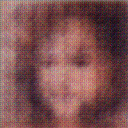
\includegraphics[width=150px]{500_fake_images/samples_5_115.png}%
\caption{A Close Up Of A Person Wearing A Tie}%
\end{figure}

%
\end{document}